\documentclass[aspectratio=43]{beamer}
\usepackage[english]{babel}
\setlength{\parskip}{\baselineskip} 
% add any packages that you need below
\usepackage{tabto}
\usepackage{float}
\usepackage{graphicx}
\usepackage{hyperref}
\usepackage[english]{babel}
\usepackage{fancyhdr}
\usepackage{titlepic}
\usepackage{parskip}
\usepackage{multirow}
\usepackage{subcaption}
\usepackage{pdfpages}
\usepackage{amsthm}
\usepackage{mathtools}
\usepackage{physics}
\usepackage{soul}
\usepackage{calligra}
\usepackage{csquotes}
\usepackage{tensor}
\usepackage[thicklines]{cancel}
\usepackage{tcolorbox}
\usepackage{pstricks}
\usepackage[backend=biber, bibstyle=nature, sorting=nty, citestyle=numeric-comp]{biblatex} 
    \addbibresource{bib.bib} 


\DeclareMathAlphabet{\mathcalligra}{T1}{calligra}{m}{n}
\DeclareFontShape{T1}{calligra}{m}{n}{<->s*[2.2]callig15}{}
\newcommand{\scriptr}{\mathcalligra{r}\,}
\newcommand{\boldscriptr}{\pmb{\mathcalligra{r}}\,}
\def\rc{\scriptr}
\def\brc{\boldscriptr}
\def\hrc{\hat\brc}
\newcommand{\ie}{\emph{i.e.}} 
\newcommand{\eg}{\emph{e.g.}} 
\newcommand{\rtd}[1]{\ensuremath{\left\lfloor #1 \right\rfloor}}
\newcommand{\dirac}[1]{\ensuremath{\delta \left( #1 \right)}}
\newcommand{\diract}[1]{\ensuremath{\delta^3 \left( #1 \right)}}
\newcommand{\e}{\ensuremath{\epsilon_0}}
\newcommand{\m}{\ensuremath{\mu_0}}
\newcommand{\V}{\ensuremath{\mathcal{V}}}
\newcommand{\prnt}[1]{\ensuremath{\left(#1\right)}} %parentheses
\newcommand{\colch}[1]{\ensuremath{\left[#1\right]}} %square brackets
\newcommand{\chave}[1]{\ensuremath{\left\{#1\right\}}}  %curly brackets

\useoutertheme{infolines}
\useinnertheme{rectangles}
\usefonttheme{professionalfonts}

% to change colours just find any references to that colour in this preamble and change it's name (you will also need to define and name your new colour below)
\definecolor{darkblue}{HTML}{151B8D} % so to change this colour give it a new name and put the colour code, then change all occurances of this colour in the rest of this preamble document to your new colour name.
\definecolor{gray}{HTML}{303030}
\definecolor{periwinkle}{HTML}{ccccff}
\definecolor{lightmauve}{HTML}{dcd0ff}

\renewcommand{\CancelColor}{\color{darkblue}}

\makeatletter
\newcommand{\mybox}[1]{
  \setbox0=\hbox{#1}
  \setlength{\@tempdima}{\dimexpr\wd0+13pt}%
  \begin{tcolorbox}[colback=darkblue,colframe=darkblue,boxrule=0.5pt,arc=4pt,
      left=6pt,right=6pt,top=6pt,bottom=6pt,boxsep=0pt,width=\@tempdima]
    \textcolor{black}{#1}
  \end{tcolorbox}
}
\makeatother

\usecolortheme[named=darkblue]{structure}
\usecolortheme{sidebartab}
\usecolortheme{orchid}
\usecolortheme{whale}
\setbeamercolor{alerted text}{fg=lightmauve}
\setbeamercolor{block title alerted}{bg=alerted text.fg!70!black}
\setbeamercolor{block title example}{bg=darkblue!60!black}
\setbeamercolor{background canvas}{bg=white}
\setbeamercolor{normal text}{bg=white,fg=black}

\setbeamertemplate{footline}
        {
      \leavevmode%
      \hbox{%
      \begin{beamercolorbox}[wd=.5\paperwidth,ht=2.25ex,dp=1ex,center]{title in head/foot}%
        \usebeamerfont{title in head/foot}\insertshorttitle
      \end{beamercolorbox}%
      \begin{beamercolorbox}[wd=.5\paperwidth,ht=2.25ex,dp=1ex,center]{date in head/foot}%
        \usebeamerfont{date in head/foot}\insertframenumber{} / \inserttotalframenumber%\hspace*{2em}

    %turning the next line into a comment, erases the frame numbers
        %\insertframenumber{} / \inserttotalframenumber\hspace*{2ex} 

      \end{beamercolorbox}}%
      \vskip0pt%
    }


\setbeamertemplate{blocks}[rectangle]
\setbeamercovered{dynamic}

\setbeamertemplate{section page}
{
	\begin{centering}
		\begin{beamercolorbox}[sep=27pt,center]{part title}
			\usebeamerfont{section title}\insertsection\par
			\usebeamerfont{subsection title}\insertsubsection\par
		\end{beamercolorbox}
	\end{centering}
}

%\setbeamertemplate{subsection page}
%{
%	\begin{centering}
%		\begin{beamercolorbox}[sep=12pt,center]{part title}
%			\usebeamerfont{subsection title}\insertsubsection\par
%		\end{beamercolorbox}
%	\end{centering}
%}

\newcommand{\hlight}[1]{\colorbox{violet!50}{#1}}
\newcommand{\hlighta}[1]{\colorbox{violet!50}{#1}} % to edit any formatting aspects of the document you need to edit this preamble document

\title[Presentation title]{Presentation title} % the bit in square brackets goes in the bar at the bottom of the slides
\author[G. Carmichael]{Grace Carmichael}
\institute[UCT]{
    Department of Statistical Sciences%
    \\
    University of Cape Town
} 
\titlegraphic{

\includegraphics[width=2cm]{logo.png}
}

\date{2025}


\begin{document}

    \frame{\titlepage} % This adds the title page to your presentation
    
    \begin{frame}{Outline} % you can remove this frame if you don't want the outline slide included
        \tableofcontents
    \end{frame}
    
    \section{Introduction to problem}
\frame{\sectionpage} % this adds the slide with the section title, if you don't want that slide included you can remove it.
    
\begin{frame}{Introduction}
\begin{itemize}
    \item Itemize lets you add bullets to your document like this.
    \item You can have as many bullets as will fit on a page.
\end{itemize}
\end{frame}

\begin{frame}{Including figures}
You can add figures/images to the document the same as you do in any latex document.  

\begin{figure}[H]
     \centering
     \begin{subfigure}[b]{0.49\linewidth}
        \centering
        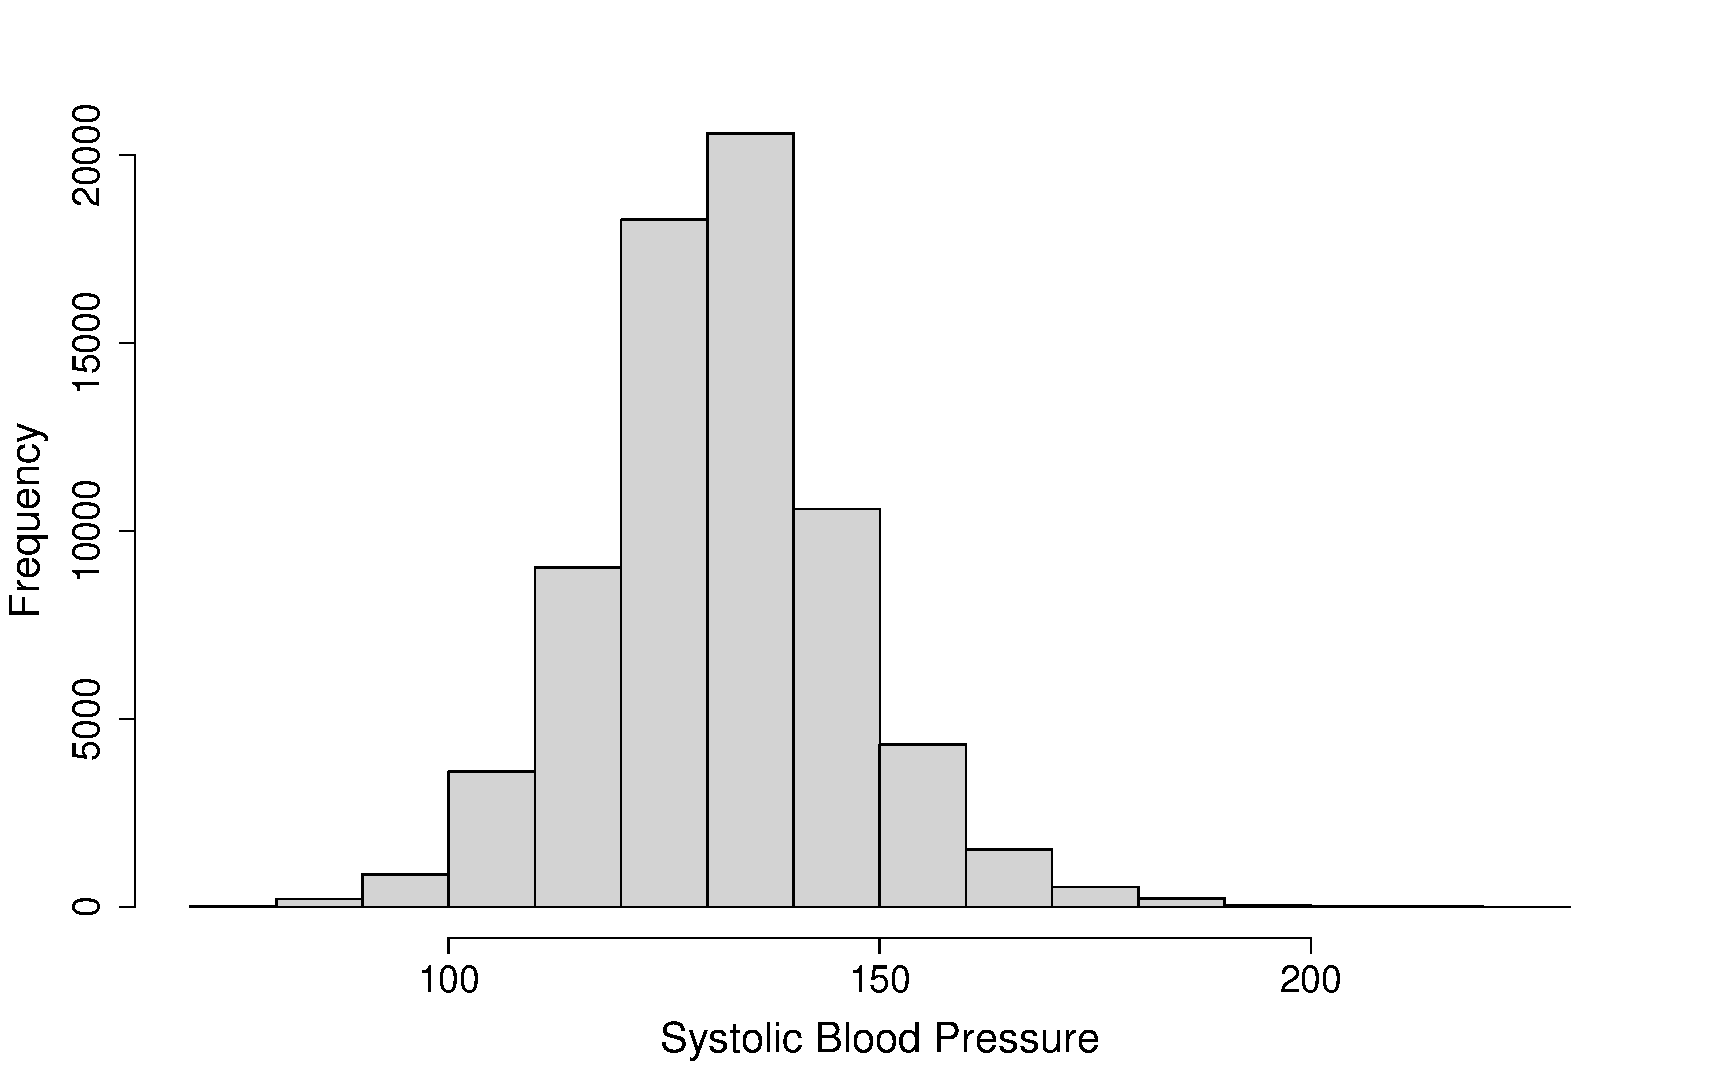
\includegraphics[width=\linewidth]{Images/hist_sys.pdf}
        \caption{Distribution of Systolic blood pressure measures.}
        \label{fig:hist_sys}
     \end{subfigure}
     \hfill
     \begin{subfigure}[b]{0.49\linewidth}
        \centering
        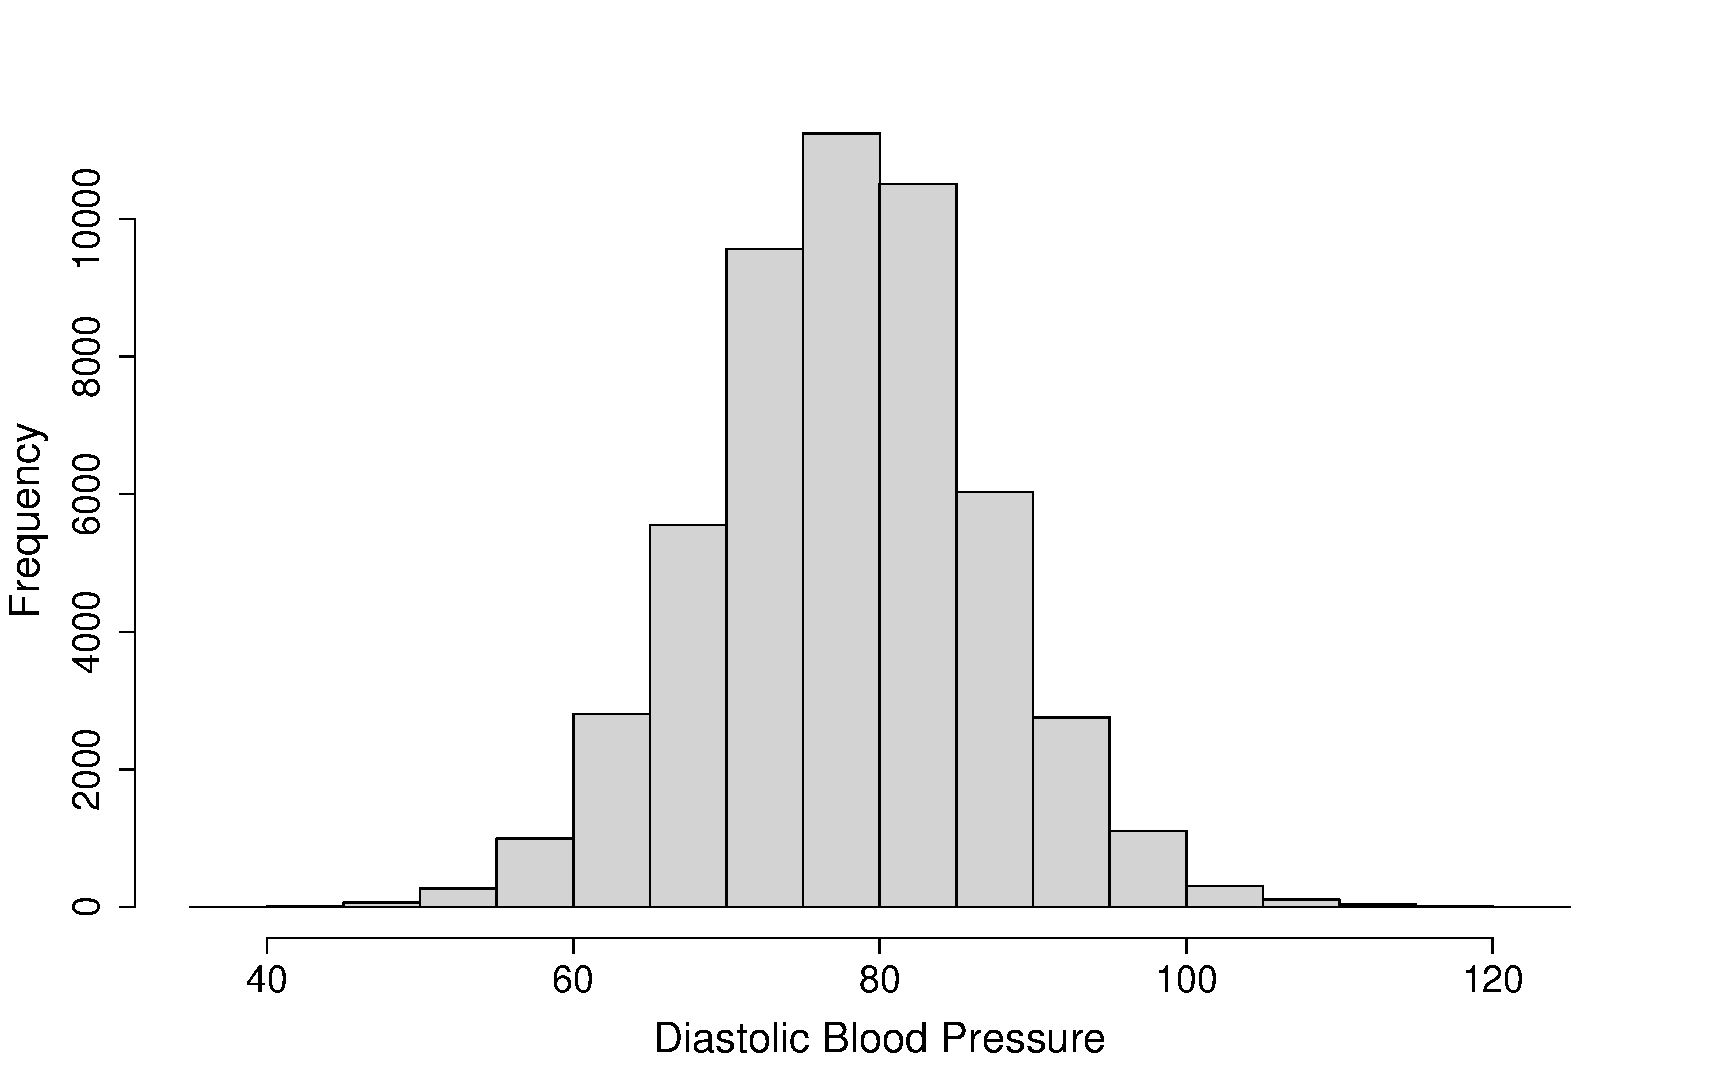
\includegraphics[width=\linewidth]{Images/hist_dia.pdf}
        \caption{Distribution of Diastolic blood pressure measures.}
        \label{fig:hist_dia}
     \end{subfigure}
     \caption{Blood pressure distributions.}
     \label{fig:hist_long}
\end{figure}

\end{frame}

\begin{frame}{Including tables}
You can add tables to the document the same as you do in any latex document.  

\begin{table}[H]
    \centering
    \caption{Intercept and Slope estimates from the linear regression model.}
    \begin{tabular}{rrrr}
    \hline
     & \textbf{Estimate} & \textbf{p-value} & \textbf{95\% CI} \\
    \hline
    \textbf{Intercept} & -1.237 & 0.324 & [-3.026 ; 0.990]\\
    \textbf{Slope} & -7.032 & 0.015 & [-12.555 ; -1.509] \\
    \hline
    \end{tabular}
    \label{tab:reg_est}
\end{table}

\end{frame}


\begin{frame}{Including equations/mathematics}
Numbered:
\begin{equation}
    \hat{y}_i = \hat{\beta}_0 + \hat{\beta}_1 x_{1i} + \hat{\beta}_{2} x_{2i} +...+ \hat{\beta}_p x_{pi}
\end{equation}
or not numbered:
\begin{equation*}
    \hat{y}_i = \hat{\beta}_0 + \hat{\beta}_1 x_{1i} + \hat{\beta}_{2} x_{2i} +...+ \hat{\beta}_p x_{pi}
\end{equation*}

You can also include maths in-line (for example: $\hat{\beta_1} = 0.53$) using dollar signs.

\end{frame} 

\end{document}
